\section{Introducción al radar}
\subsection{Espectro electromagnético}
\begin{frame}{\secname : \subsecname}
  \begin{figure}
    \centering
    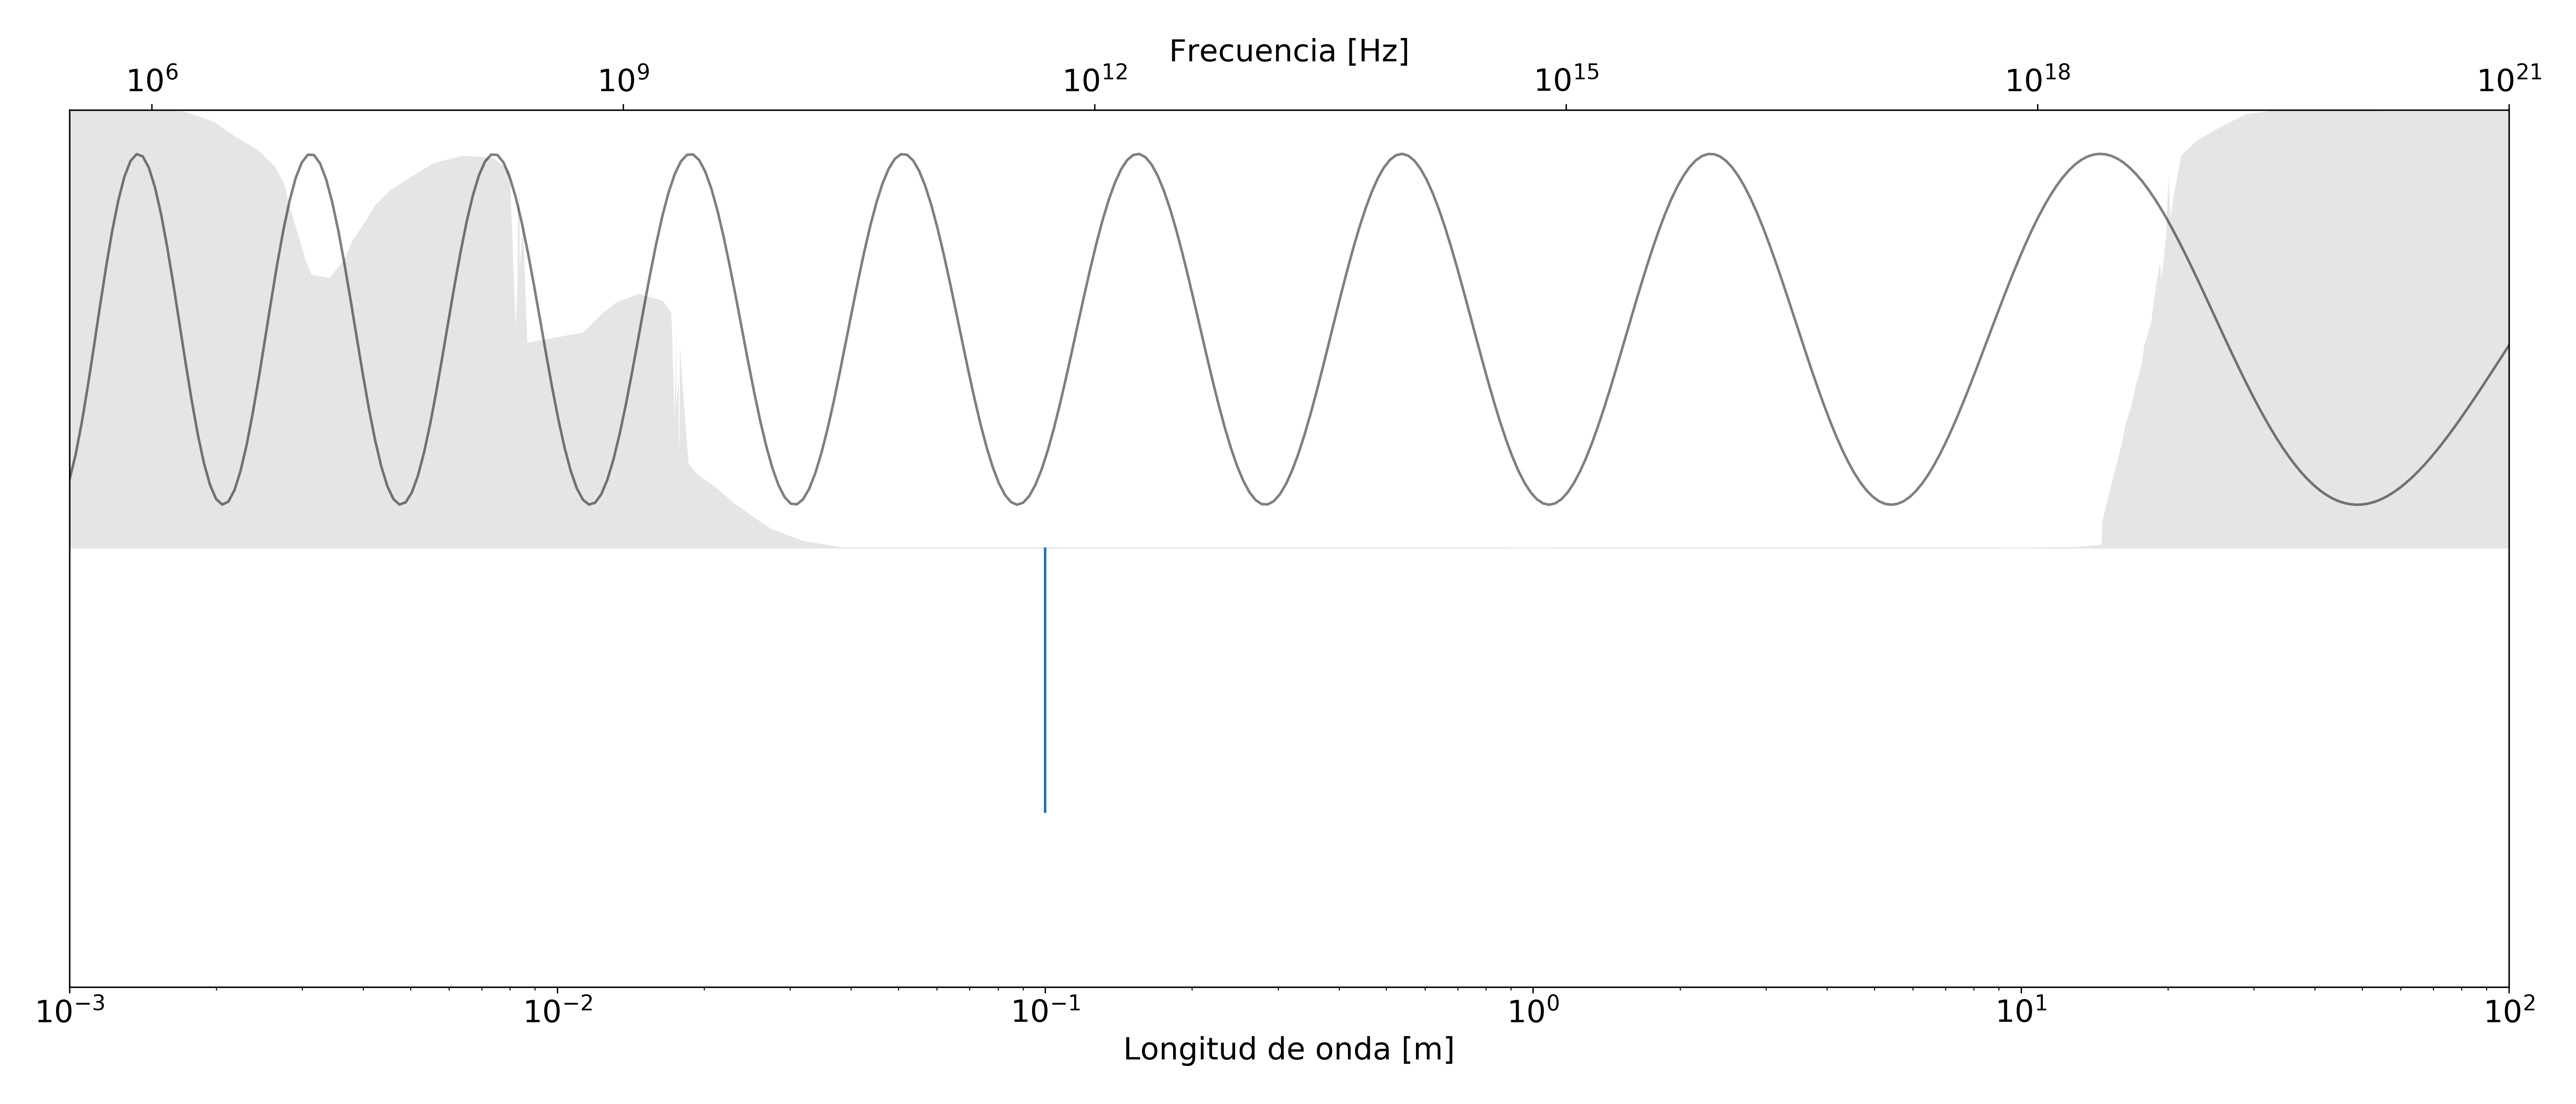
\includegraphics[width=\textwidth]{fig:espectro.png}
    \caption{Espectro electromagnético en longitud de onda (abajo) y frecuencia (arriba).}
    \label{}
  \end{figure}
\end{frame}
%--- Next Frame ---%

\subsection{¿Qué es un radar?}
\begin{frame}{\secname : \subsecname}
    \begin{figure}
      \centering
      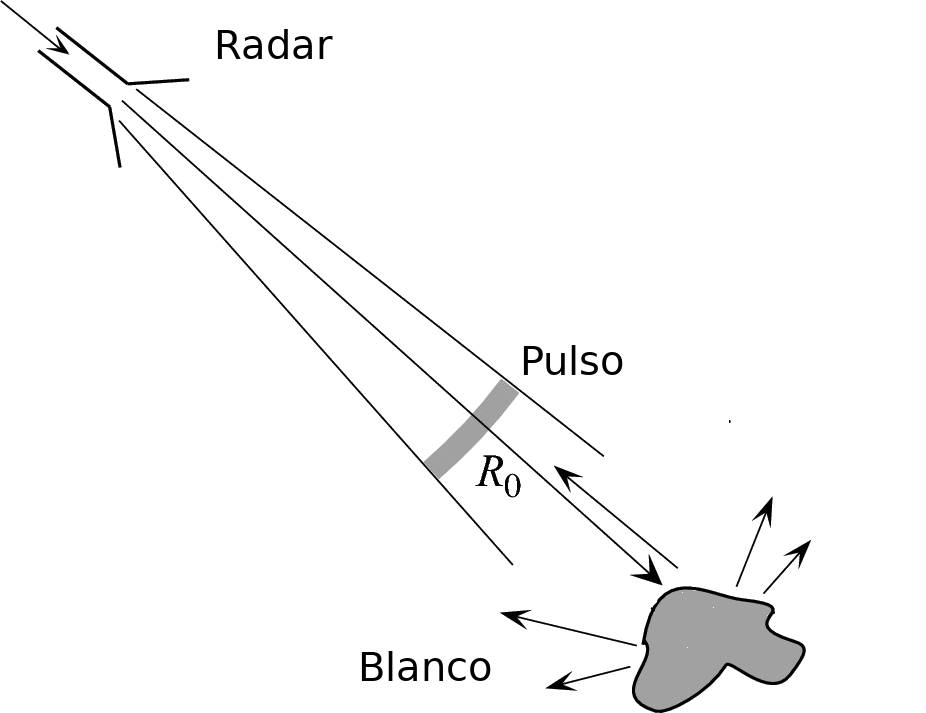
\includegraphics[scale=0.7]{fig:radar.png}
      \caption{RAdio Detection And Ranging. Funcionamiento esquemático.}
      \label{}
    \end{figure}
\end{frame}
%--- Next Frame ---%

\subsection{¿Cómo detecta un radar?}
\begin{frame}{\secname : \subsecname}
  \begin{figure}
    \centering
    \movie[width = \textwidth,loop,autostart]{\centering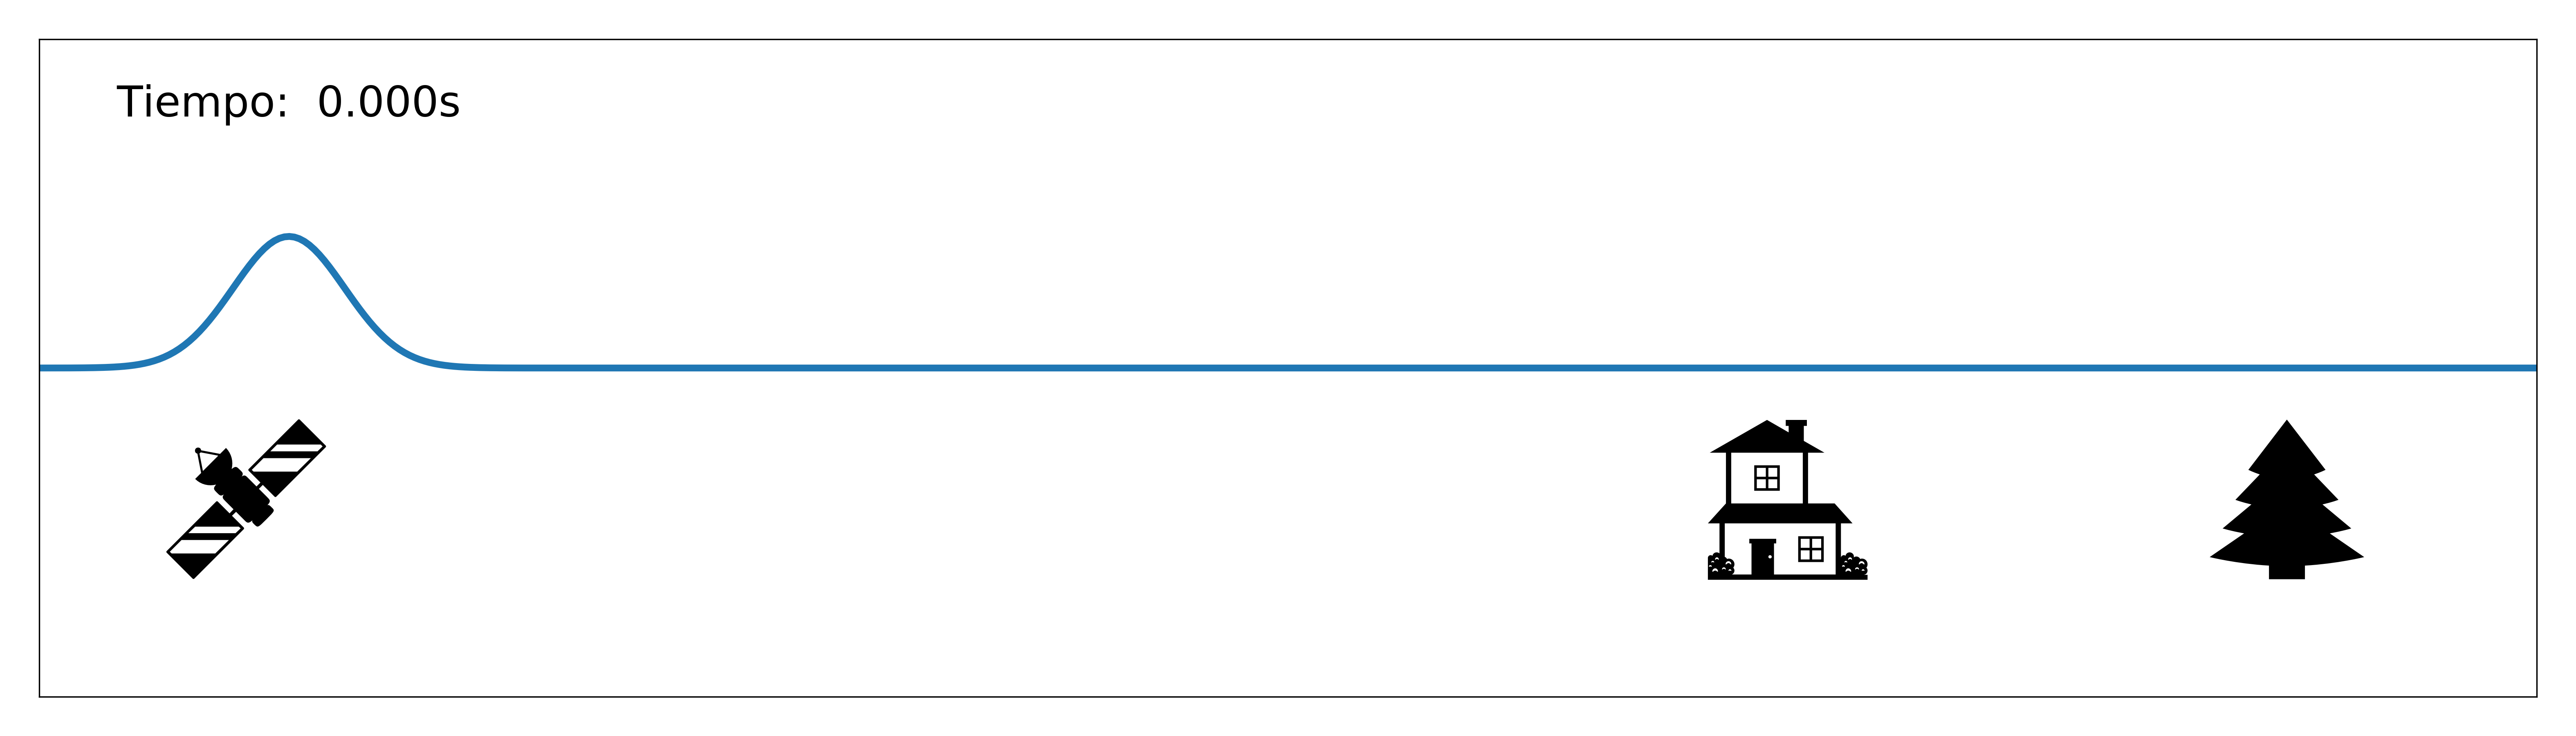
\includegraphics[width=\textwidth]{fig:funcionamiento.png}}{./figs/fig:funcionamiento.mp4}
    \caption{Ecos detectados por un radar en función del tiempo}
    \label{}
  \end{figure}
\end{frame}
%--- Next Frame ---%

\subsection{Ecuación de radar}
\begin{frame}{\secname : \subsecname}
    \begin{block}{Definición}
      \begin{equation}
        P_r = \frac{P_t G_t G_r \lambda^2 \sigma}{(4\pi)^3 R^4}
      \end{equation}
      Con $P_r$ y $P_t$ las las potencias recibidas y transmitidas, $G_r$ y $G_t$ las ganancias del emisor y receptor, $\lambda$ la longitud de onda, $\sigma$ el coeficiente de backscatter y $R$ la distancia entre el emisor y el blanco.
    \end{block}
\end{frame}
%--- Next Frame ---%

\subsection{decibels}
\begin{frame}{\secname : \subsecname}
    \begin{block}{Definición}
      Es común expresar la potencia de un radar en decibels cómo
      \begin{equation}
        P [dB] = 10\log_{10}\left( \frac{P}{P_0}\right)
      \end{equation}
      donde $P_0$ es una potencia de referencia.
    \end{block}
\end{frame}
%--- Next Frame ---%

\subsection{Generación de una imagen}
\begin{frame}{\secname : \subsecname}
  \begin{figure}
    \centering
    \movie[width = 0.95\textwidth,loop,autostart]{\centering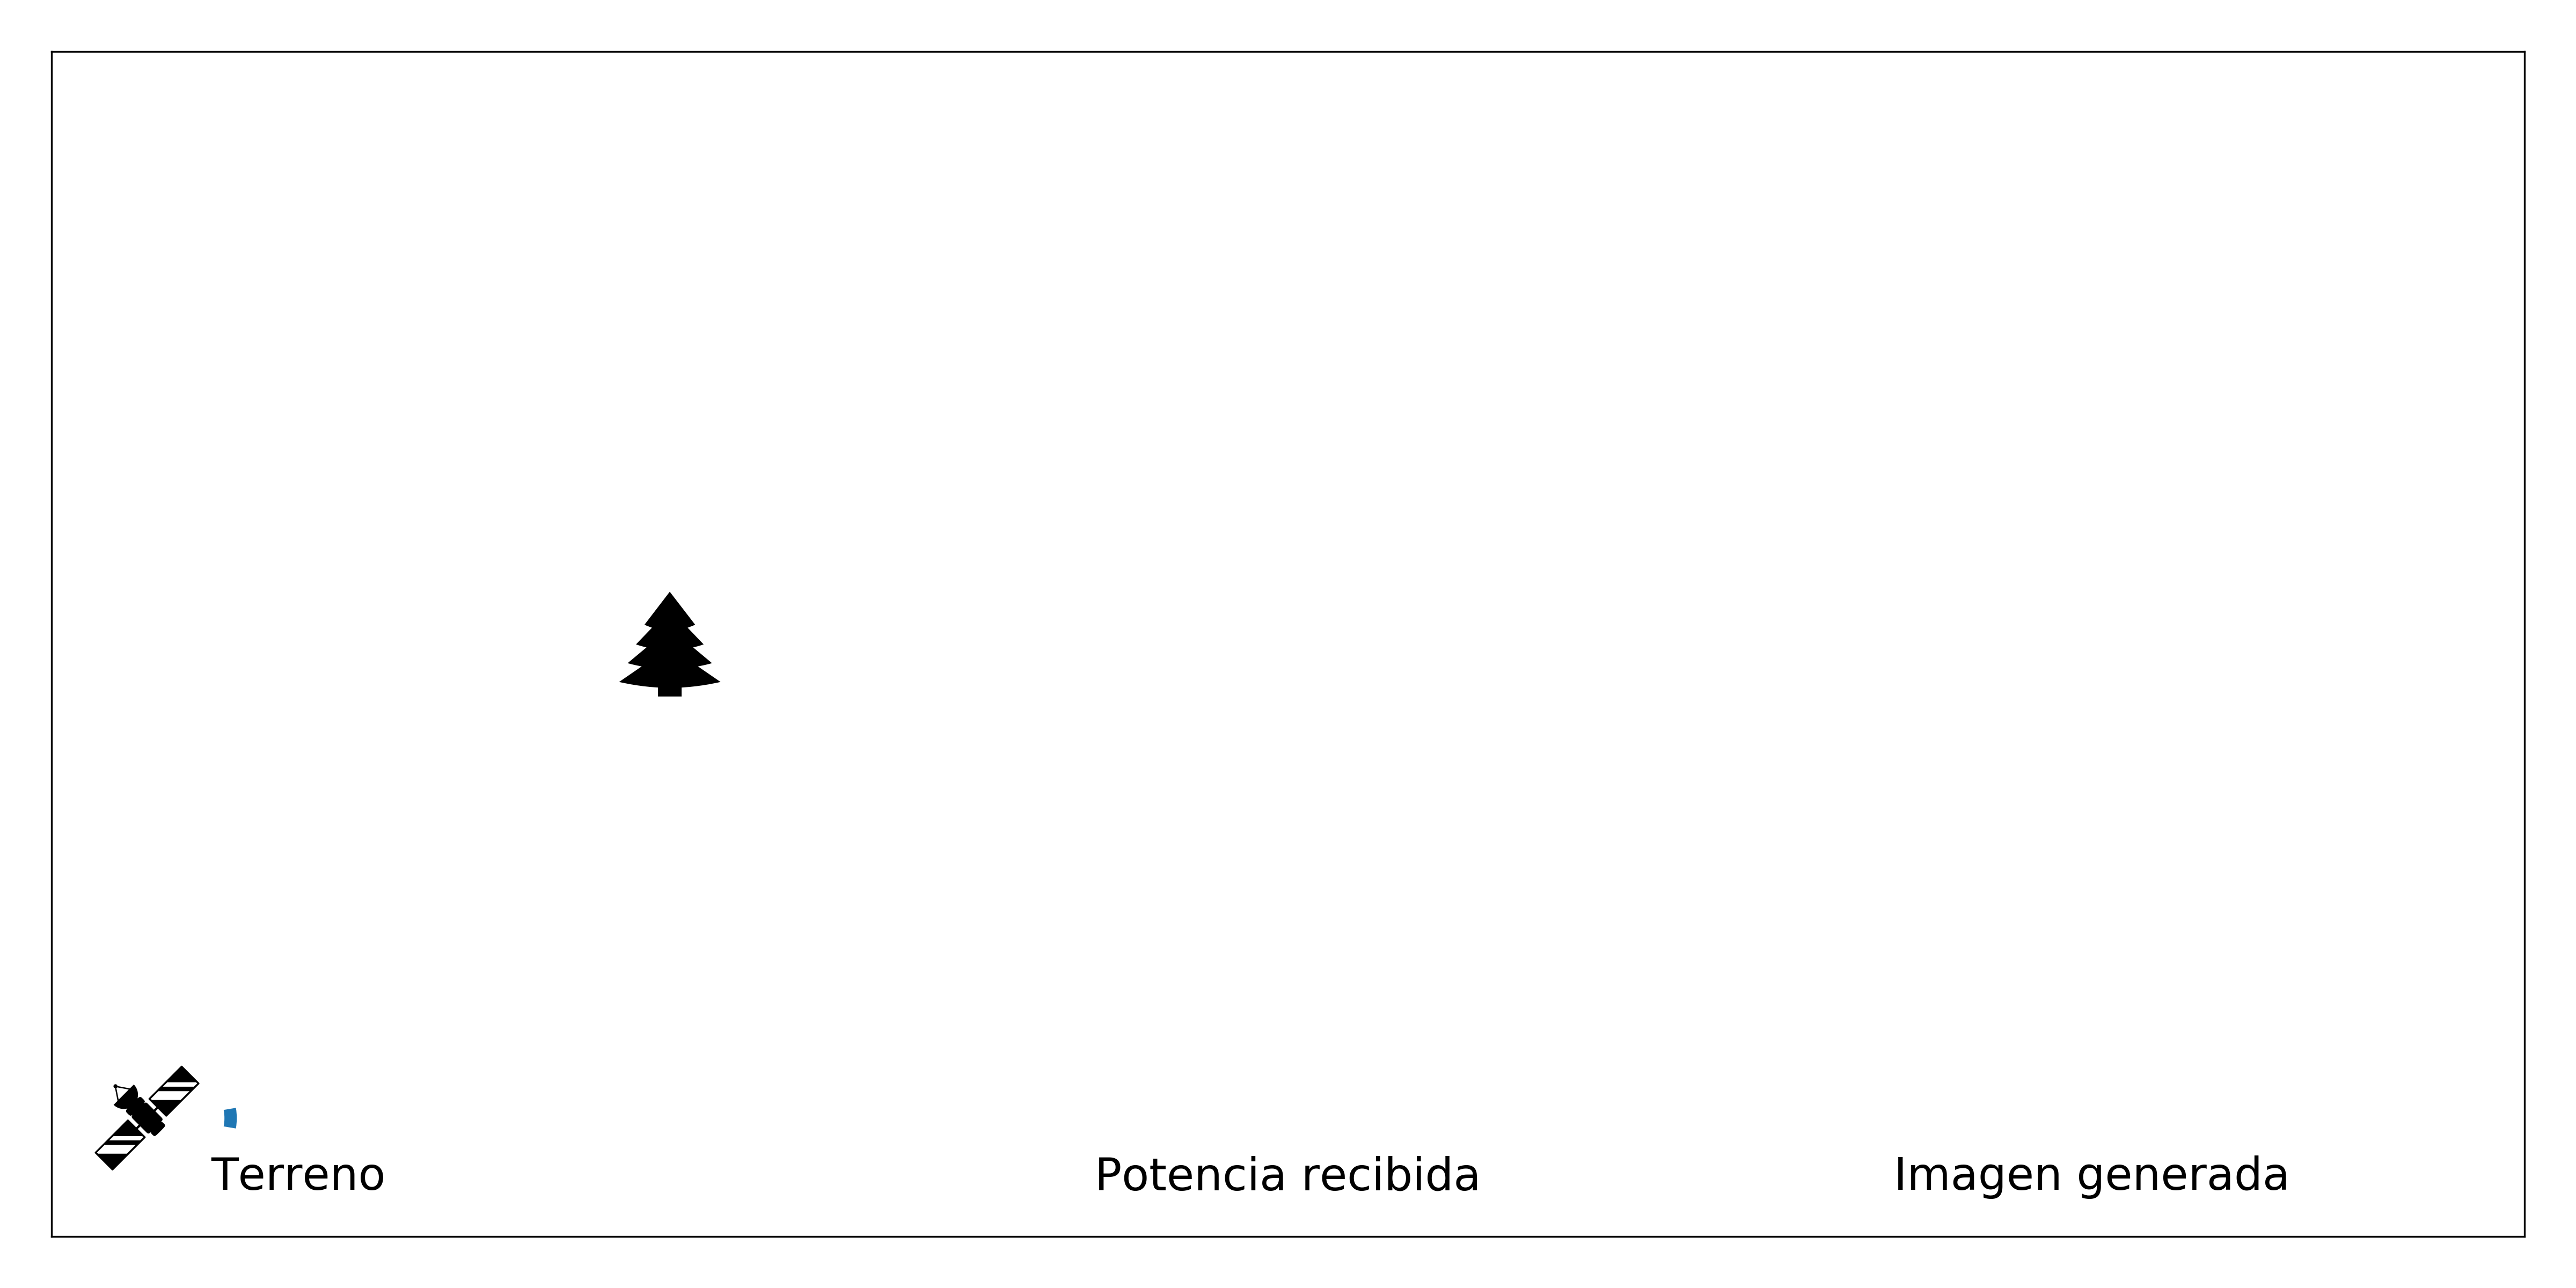
\includegraphics[width=0.95\textwidth]{fig:imagen.png}}{./figs/fig:imagen.mp4}
    \caption{Generación de una imagen radar a partir de datos en el terreno.}
    \label{}
  \end{figure}
\end{frame}
%--- Next Frame ---%

\subsection{Geometría}
\begin{frame}{\secname : \subsecname}
  \begin{figure}
    \centering
    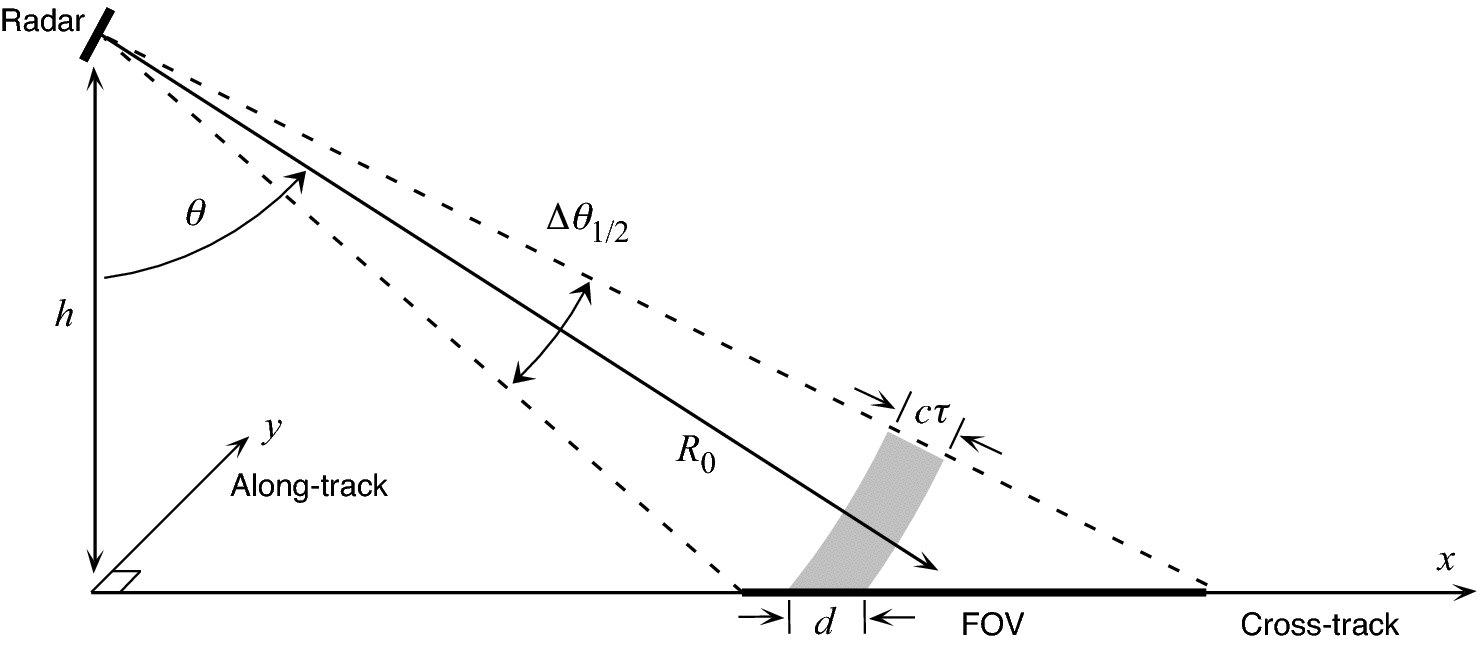
\includegraphics[scale=0.7]{01938fig10_3.jpg}
    \caption{Geometría de observación de un radar en dos dimensiones viso en un corte transversal.}
    \label{}
  \end{figure}
\end{frame}
%--- Next Frame ---%

\begin{frame}{\secname : \subsecname}
  \begin{figure}
    \centering
    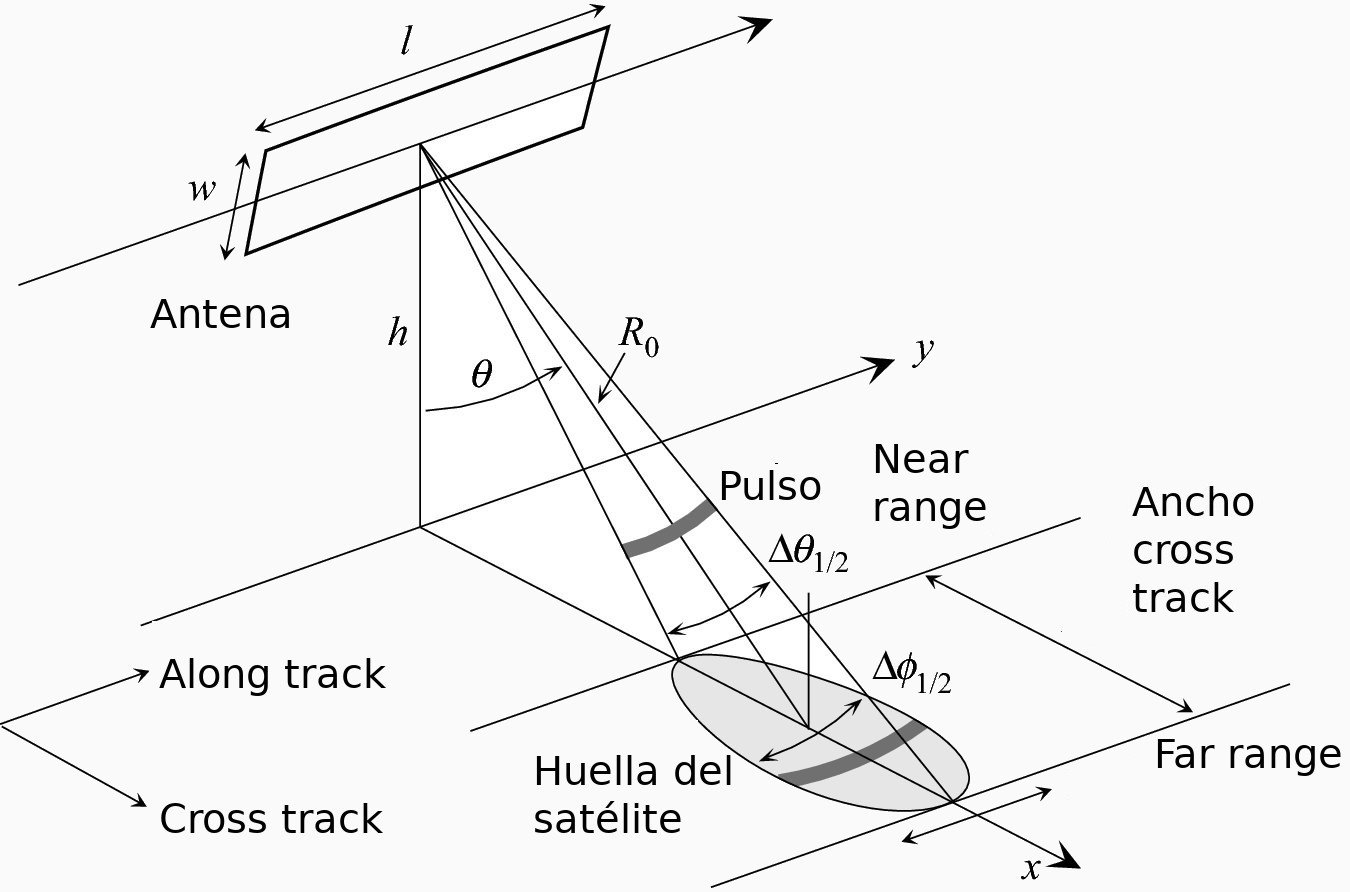
\includegraphics[scale=0.7]{01938fig13_1.jpg}
    \caption{Geometría de observación de un radar completa en la direcciones perpendiculares y paralelas al movimiento (accross track y along track)}
    \label{}
  \end{figure}
\end{frame}
%--- Next Frame ---%

\subsection{Modos de adquisición}

\begin{frame}{\secname : \subsecname}
    \begin{block}{SCANSAR}
      \begin{itemize}
        \item El RADAR Va distribuyendo pulsos de  a bursts entre varios swaths
        \item Gran swath
        \item Baja resolución
        \item Mala relación señal ruido en algunas partes y buena en otras
        \item Mala distribución de potencia generando scalloping
        \item Un poco mas complicado de procesar
        \item Hace falta reapuntar la antena en elevación entre burst
      \end{itemize}
    \end{block}
\end{frame}
%--- Next Frame ---%

\begin{frame}{\secname : \subsecname}
    \begin{block}{TOPSAR}
      \begin{itemize}
        \item El RADAR Va distribuyendo pulsos entre varios swaths y variando el apuntamiento en acimut para iluminar la pisada de manera mas homogénea
        \item Gran swath
        \item Baja resolución
        \item Aceptable relación señal ruido y uniforme en la imagen.
        \item Buena distribución de potencia. No hay scalloping
        \item Un poco mas complicado de procesar
      \end{itemize}
    \end{block}
\end{frame}
%--- Next Frame ---%

\subsection{Comparación con el óptico}
\begin{frame}{\secname : \subsecname}
\begin{columns}
  \begin{column}{0.5\textwidth}
   \begin{block}{Óptico}
     \begin{itemize}
       \item Rango de trabajo en los micrometros ($0.3\mu$ m a $2.5\mu m$).
       \item Detecta luz solar reflejada por la tierra.
       \item Bloqueado por las nubes.
       \item Detecta luz incoherente.
       \item Depende de una fuente de iluminación externa.
     \end{itemize}
   \end{block}
  \end{column}
  \begin{column}{0.5\textwidth}  %%<--- here
    \begin{block}{Radar}
      \begin{itemize}
        \item Rango de trabajo en los microondas ($1cm$ m a $100cm$).
        \item Emite una señal y mide la intesidad del eco.
        \item Independiente de las condiciones atmosféricas.
        \item Emite y detecta una onda coherente.
        \item Cuenta con su propia fuente de iluminación.
      \end{itemize}
    \end{block}
  \end{column}
  \end{columns}
\end{frame}
%--- Next Frame ---%
